\chapter{直流-直流変換(2) 絶縁型}
\label{chap6}

5章では，スイッチとインダクタ・キャパシタだけで直流電圧を変える
非絶縁型のDC-DCコンバータを学んだ。
しかし，コンセントにつながる機器の電源には，5章の回路をそのまま使えない。
入力と出力が導線でつながったままでは，感電の危険を断ち切れないからである。
本章では，入力と出力の間を\textbf{変圧器（トランス）}で切り離した
\textbf{絶縁型}のDC-DCコンバータを学ぶ。
といっても，新しい理屈が増えるわけではない。
5章で使った道具 ― オン・オフ2つの等価回路と\textbf{ボルト秒平衡} ― を，
トランス込みでもう一度使うだけである。
本章ではまず絶縁がなぜ必要かを整理し（\ref{sec6.1}節），
トランスの物理を励磁電流と\rev{反射電流}の分離という形でつかむ（\ref{sec6.2}節）。
そのうえで，絶縁型降圧のフォワードコンバータ（\ref{sec6.3}節）と
絶縁型昇降圧のフライバックコンバータ（\ref{sec6.4}節）を解析する。

\begin{screen}
\noindent\textbf{本章の現在地}\\[3pt]
序章の地図（\ref{fig0.1}）では直流→直流（DC-DC変換，5〜7章）の2章目にいる。
エネルギーの視点でいえば，本章の回路はどちらも
\textbf{エネルギーを一度トランスに預けて渡す}回路である。
ただし預け方が対照的で，
\textbf{フォワードはオンの間にトランスを素通しで渡し，
フライバックはオンの間にトランスへ溜めて，オフの間に渡す}。
この対比が本章の背骨である。
\end{screen}

%%======================================================================
\section{絶縁の必要性とメリット}
\label{sec6.1}

\subsection{絶縁とは何か}

\index{ぜつえん@絶縁}\textbf{絶縁}とは，入力側と出力側の間に
導線による電流の通り道がないことをいう。
入力と出力を絶縁したうえでエネルギーだけを受け渡す変換器を
\index{ぜつえんがたこんばーた@絶縁型コンバータ}\textbf{絶縁型コンバータ}という。
5章の降圧・昇圧・昇降圧コンバータは，入力の負極と出力の負極が
導線で直結していた。これらは非絶縁型である。
%% [対応済 2026-09-08] 著者指摘（絶縁型もチョッパである）: 5.1節の分類を2軸に改めたのに合わせ，
%%   絶縁型も方式としてはチョッパであることをここで断った。
スイッチで刻んで平均値を制御するという点では，本章の回路も5章と同じである。
どちらもスイッチング方式の変換回路であり，違いは変圧器を挟むかどうかだけである
（\ref{chap5}章\ref{sec5.1}節の分類を見よ）。

導線を切り離してどうやってエネルギーを渡すのか。
その橋渡し役が変圧器である。
変圧器は2つの巻線を磁気的に結び付けた素子で，
電流の通り道はつながっていないのに，
磁束を仲立ちとしてエネルギーを渡すことができる。

\subsection{なぜ絶縁が必要か}

絶縁のメリットは3つある。

第一に\textbf{感電\index{かんでん@感電}からの保護}である。
コンセントの交流100\,Vは，柱上変圧器のところで片側が大地に接続されている。
このため非絶縁型では，\FIGref{fig6.1}(a)のように出力端子と大地の間に
商用電源の電位差がそのまま現れる場所ができ，
出力側の金属部分に触れると感電するおそれがある。
絶縁型では\ref{fig6.1}(b)のように出力側が入力側の電位から切り離されるので，
出力側のどこか1点を安心して大地や筐体につなぎ，
新しい基準電位を自由に決められる。

\begin{figure}[ht]
\begin{center}
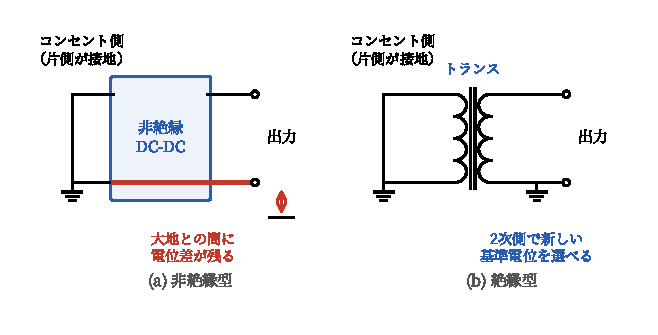
\includegraphics[clip]{figures/fig6.1.eps}
\end{center}
\caption{絶縁の役割。(a)非絶縁型では出力端子が入力側の電位を引きずり，
大地との間に商用電源の電位差が現れる。(b)絶縁型ではトランスが電流の道を断ち切り，
2次側で新しい基準電位を選べる}
\label{fig6.1}
\end{figure}

第二に\textbf{電位差の遮断}である。
機器と機器をつなぐと，それぞれの基準電位（グラウンド）が
一致しているとは限らず，基準電位の差が電流やノイズとなって回り込む。
絶縁はこの回り込みの道そのものを断ち切る。
医療機器や通信機器で絶縁が必須とされる理由である。

第三に\textbf{巻数比\index{まきすうひ@巻数比}による大比率の変換}である。
次節で見るように，変圧器は巻数の比で電圧を変えられる。
5章の降圧コンバータでも出力電圧はデューティ比$D$でいくらでも下げられるはずだが，
変換比が大きいと$D$が極端に小さくなり，
オン時間がスイッチの切替え時間に近づいて制御が難しくなる。
絶縁型では，大まかな変換は巻数比に受け持たせ，
$D$は制御しやすい0.3〜0.5前後で微調整に使う，という分担ができる。

\begin{問}
\item AC100\,Vを整流すると約$141$\,Vの直流が得られる（8章）。
ここから$5$\,Vを作るとき，5章の降圧コンバータ（$V_{\mathrm{out}} = D V_{\mathrm{in}}$）では
デューティ比$D$がいくつになるか。
スイッチング周波数$100$\,kHzのときのオン時間を求め，
スイッチの切替えに数十\,nsかかることと比べて何が起こるか述べよ。
\end{問}

\rev{大まかな変換は巻数比，微調整はデューティ比 ― この分担を支える変圧器の物理を，次節で4章のインダクタの延長として押さえる。}

%%======================================================================
\section{変圧器の基礎物理}
\label{sec6.2}

\subsection{電圧は巻数に比例する}

\index{へんあつき@変圧器}\textbf{変圧器}は，
1つの鉄心に2つの巻線を巻いた素子である（\FIGref{fig6.2}(a)）。
入力側の巻線を\index{01じまきせん@1次巻線}\textbf{1次巻線}（巻数$N_1$），
出力側を\index{02じまきせん@2次巻線}\textbf{2次巻線}（巻数$N_2$）という。
鉄心は磁束の通り道であり，磁束は漏れずに全部が両方の巻線を貫くとする。

1次巻線に電圧$v_1$を加えると，
電磁誘導の法則（4章）により鉄心内の磁束$\mathit{\Phi}$が変化する。
巻線は磁束を$N_1$回貫かれているから
\begin{equation}
v_1 = N_1 \frac{d\mathit{\Phi}}{dt}
\label{eq6.1}
\end{equation}
である。同じ磁束$\mathit{\Phi}$は2次巻線も$N_2$回貫くので，2次側には
\begin{equation}
v_2 = N_2 \frac{d\mathit{\Phi}}{dt}
\label{eq6.2}
\end{equation}
の電圧が誘導される。式\ref{eq6.1}と式\ref{eq6.2}から$d\mathit{\Phi}/dt$を消去すると
\begin{equation}
\frac{v_2}{v_1} = \frac{N_2}{N_1}
\label{eq6.3}
\end{equation}
となる。\textbf{電圧の比は巻数の比で決まる}。
これが変圧器の第一の顔である。

\begin{figure}[ht]
\begin{center}
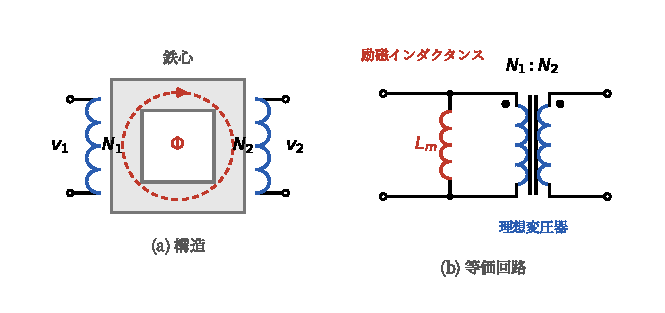
\includegraphics[clip]{figures/fig6.2.eps}
\end{center}
\caption{変圧器の構造と等価回路。(a)鉄心を貫く磁束$\mathit{\Phi}$が2つの巻線を結び，
(b)等価回路では磁束を作る役割を励磁インダクタンス$L_m$が，
電圧・電流の変換を理想変圧器が受け持つ}
\label{fig6.2}
\end{figure}

\subsection{励磁電流 ― 磁束を作る電流}

電圧の関係だけなら式\ref{eq6.3}で済むが，電流はそう単純ではない。
2次側に何もつながず開放したままでも，1次巻線に電圧をかければ電流が流れる。
式\ref{eq6.1}のとおり磁束が変化し続けるためには，
磁束を作る電流が必要だからである。

\begin{定義}[励磁電流と励磁インダクタンス]
\label{def6.1}
鉄心の磁束を作るために1次巻線を流れる電流を
\index{れいじでんりゅう@励磁電流}\textbf{励磁電流}$i_m$という。
磁束は励磁電流に比例し（$N_1\mathit{\Phi} = L_m i_m$），比例係数$L_m$を
\index{れいじいんだくたんす@励磁インダクタンス}\textbf{励磁インダクタンス}という。
式\ref{eq6.1}に代入すれば
\begin{equation}
v_1 = L_m \frac{di_m}{dt}
\label{eq6.4}
\end{equation}
となり，1次側から見た変圧器は1つのインダクタとして振る舞う。
\end{定義}

つまり\textbf{変圧器も磁気エネルギーを蓄える素子}であり，
励磁電流$i_m$は4章のインダクタとまったく同じ式\ref{eq6.4}に従って，
エネルギー$\frac{1}{2}L_m i_m^2$を鉄心の磁場に蓄えている。
ここが本章の急所である。
インダクタと同じ式に従う以上，5章で学んだボルト秒平衡
\index{ぼるとびょうへいこう@ボルト秒平衡} ―
定常状態では1周期にわたる電圧の平均がゼロ ― は，
\textbf{励磁インダクタンスにもそのまま要求される}。
正の電圧ばかりかけ続ければ$i_m$と磁束は増える一方で，
やがて鉄心の磁束が上限に達して
\index{じきほうわ@磁気飽和}\textbf{磁気飽和}を起こす。
飽和した鉄心はインダクタンスを失い，励磁電流が暴走して素子を壊す。
「蓄えっぱなしは許されない」 ―
この制約が\ref{sec6.3}節のリセット巻線を生み，
逆にこの蓄えを積極的に利用するのが\ref{sec6.4}節のフライバックである。

\begin{例題}[励磁電流の計算]
\label{rei6.1}
励磁インダクタンス$L_m = 1$\,mHの変圧器の1次巻線に，
$\pm10$\,V，半周期$1.0$\,$\mu$sの方形波電圧を加えた。
2次側は開放とする。定常状態の励磁電流$i_m$の波形を求めよ。
\begin{解答}
式\ref{eq6.4}より，電圧が$+10$\,Vの間，$i_m$は一定の傾き
\begin{equation*}
\frac{di_m}{dt} = \frac{v_1}{L_m} = \frac{10}{1\times10^{-3}}
= 1.0\times10^{4}\,\mathrm{A/s}
\end{equation*}
で増える。半周期$1.0$\,$\mu$sでの増加量は
\begin{equation*}
\mathit{\Delta}I_m = \frac{v_1}{L_m}\,\mathit{\Delta}t
= 1.0\times10^{4} \times 1.0\times10^{-6} = 10\,\mathrm{mA}
\end{equation*}
電圧が$-10$\,Vの半周期には同じ傾きで減る。
方形波は正負対称でボルト秒平衡が自動的に満たされるから，
$i_m$は$-5$\,mAから$+5$\,mAの間を往復する三角波になる。
電圧が方形波，電流が三角波 ― 5章のインダクタ電流と同じ形である。
\end{解答}
\end{例題}

\subsection{反射電流 ― 2次側の電流を打ち消す電流}

次に2次側に負荷をつなぐ。
2次側には式\ref{eq6.3}の電圧$v_2$が現れているから，\rev{2次側の負荷に電流$i_2$が流れる}。
ところが$i_2$も巻線を流れる電流である以上，鉄心に自分の磁束を作ろうとする。
もし磁束が変わってしまうと，式\ref{eq6.1}が電圧源$v_1$と矛盾する。
磁束は電圧源によって式\ref{eq6.1}のとおりに固定されているのである。
そこで1次側には，$i_2$の作る磁束をちょうど打ち消すだけの電流$i_{\ell}$が
追加で流れ込む。磁束を打ち消し合う条件は，巻数$\times$電流が等しいこと
\begin{equation}
N_1 i_{\ell} = N_2 i_2
\label{eq6.5}
\end{equation}
である。\rev{この$i_{\ell}$を，2次側の負荷電流が1次側に映ったものという意味で\index{はんしゃでんりゅう@反射電流}\textbf{反射電流}（1次側負荷電流）と呼ぶ。5章で負荷電流と呼んだ出力電流$I_{\mathrm{out}}$とは区別する。}
結局，1次電流は2つの成分の和になる。
\begin{equation}
i_1 = i_m + i_{\ell} = i_m + \frac{N_2}{N_1} i_2
\label{eq6.6}
\end{equation}

\FIGref{fig6.3}に，例題\ref{rei6.1}の変圧器（$N_1 = N_2$）の2次側に
抵抗$500$\,$\Omega$をつないだときの波形を示す。
2次電圧は$v_1$と同じ方形波，\rev{反射電流}$i_{\ell} = i_2 = v_2/R$は
$\pm20$\,mAの方形波，励磁電流は$\pm5$\,mAの三角波で，
1次電流$i_1$は両者の重ね合わせになっている。

\begin{figure}[ht]
\begin{center}
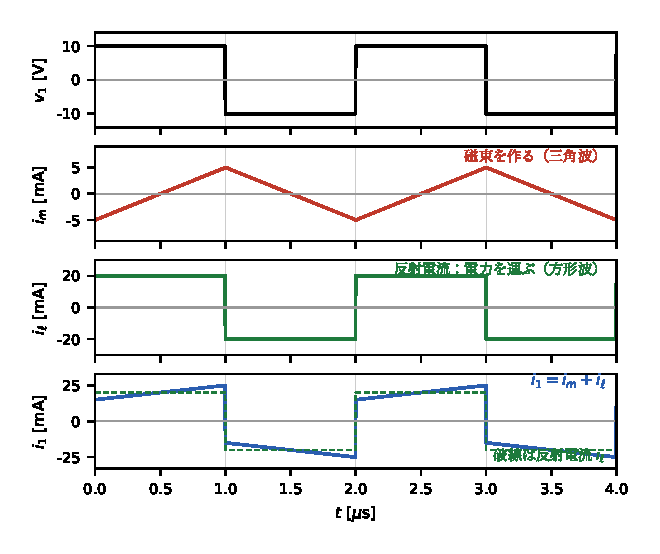
\includegraphics[clip]{figures/fig6.3.eps}
\end{center}
\caption{励磁電流と\rev{反射電流}（$N_1=N_2$，$L_m=1$\,mH，負荷500\,$\Omega$）。
1次電流$i_1$は，磁束を作る励磁電流$i_m$（三角波）と，
2次電流の磁束を打ち消す\rev{反射電流}$i_{\ell}$（方形波）の和である}
\label{fig6.3}
\end{figure}

\rev{反射電流$i_{\ell}$と2次電流$i_2$は}，磁束を互いに打ち消し合いながら
同時に流れる。つまり磁束には何も足さずに，
1次側の電力$v_1 i_{\ell} = v_2 i_2$をそっくり2次側へ手渡す。
一方，励磁電流$i_m$は負荷があってもなくても変わらず流れ，
鉄心の磁束を維持する役だけを担う。
\rev{\textbf{電力を運ぶのは反射電流，磁束を保つのは励磁電流}。}
この分離が絶縁型コンバータを読み解く鍵になる。

\begin{定義}[理想変圧器]
\label{def6.2}
励磁電流が無視できるほど$L_m$が大きく，磁束の漏れも損失もない変圧器を
\index{りそうへんあつき@理想変圧器}\textbf{理想変圧器}という。
理想変圧器では
\begin{equation}
\frac{v_2}{v_1} = \frac{N_2}{N_1}，\qquad
\frac{i_2}{i_1} = \frac{N_1}{N_2}
\label{eq6.7}
\end{equation}
が成り立ち，入力電力と出力電力は等しい（$v_1 i_1 = v_2 i_2$）。
\end{定義}

実際の変圧器は，\ref{fig6.2}(b)のように
\textbf{理想変圧器に励磁インダクタンス$L_m$を並列につないだ等価回路}で表せる。
電圧と電流の変換は理想変圧器が，磁束の維持（とエネルギーの蓄積）は
$L_m$が受け持つ，という役割分担を回路図の形にしたものである。

\begin{注意}
巻線の巻き方向によって，2次電圧の向きは反転する。
回路図では，同じ向きの電圧が現れる端子に
\index{きょくせいまーく@極性マーク}\textbf{極性マーク}（ドット）を打って区別する。
フライバックコンバータ（\ref{sec6.4}節）はこのドットの向きを
あえて逆に取ることで成り立つ回路であり，ドットを打ち間違えると動作しない。
\end{注意}

\subsection{シミュレーションでの変圧器の扱い}

LTspiceに変圧器という部品はなく，2つのインダクタ$L_1$，$L_2$を
\begin{quote}
\texttt{K1 L1 L2 1}
\end{quote}
という結合の指定で結んだ
\index{けつごういんだくた@結合インダクタ}\textbf{結合インダクタ}として表す。
末尾の1は\index{けつごうけいすう@結合係数}\textbf{結合係数}で，
1なら漏れのない理想結合である。
インダクタンスは巻数の2乗に比例するから，巻数比は
\begin{equation}
\frac{L_1}{L_2} = \left(\frac{N_1}{N_2}\right)^{\!2}
\label{eq6.8}
\end{equation}
で指定する。たとえば巻数比$10:1$なら$L_1 = 10$\,mH，$L_2 = 0.1$\,mHとする。
このとき1次側の$L_1$の値そのものが励磁インダクタンス$L_m$になる。
つまりLTspiceの変圧器モデルは，\ref{fig6.2}(b)の等価回路
（理想変圧器$+$励磁インダクタンス）を最初から含んでいる。
励磁電流を無視しない本章の議論は，そのままシミュレーションで確かめられる。

\begin{問}
\item 式\ref{eq6.1}と式\ref{eq6.4}の両辺の単位が一致することを確かめよ。
磁束の単位はWb（$1\,\mathrm{Wb} = 1\,\mathrm{V\cdot s}$），
インダクタンスの単位はH（$1\,\mathrm{H} = 1\,\mathrm{V\cdot s/A}$）である。
\end{問}

\rev{変圧器は「理想変圧器＋励磁インダクタンス」である ― この見方を手に，次節から実際のコンバータに入る。}

%%======================================================================
\section{フォワードコンバータ ― トランスを素通しで渡す}
\label{sec6.3}

\subsection{降圧コンバータにトランスを入れる}

\index{ふぉわーどこんばーた@フォワードコンバータ}\textbf{フォワードコンバータ}は，
5章の非絶縁型の降圧コンバータのスイッチと還流ダイオードの間に変圧器を挟んだ，
絶縁型の降圧コンバータである（\FIGref{fig6.4}(a)）。
オンの間，入力から2次側へ電力がトランスを素通しで（forward＝前方へ）
送られることからこの名がある。
1次側はスイッチ$\mathrm{S}$と1次巻線$N_1$，
2次側は整流ダイオード$\mathrm{D_1}$，還流ダイオード$\mathrm{D_2}$，
インダクタ$L$，キャパシタ$C$，負荷$R$で，
$\mathrm{D_1}$から後ろは5章の降圧コンバータの出力段そのものである。
リセット巻線$N_3$とダイオード$\mathrm{D_3}$の役割は後述する。

\begin{figure}[ht]
\begin{center}
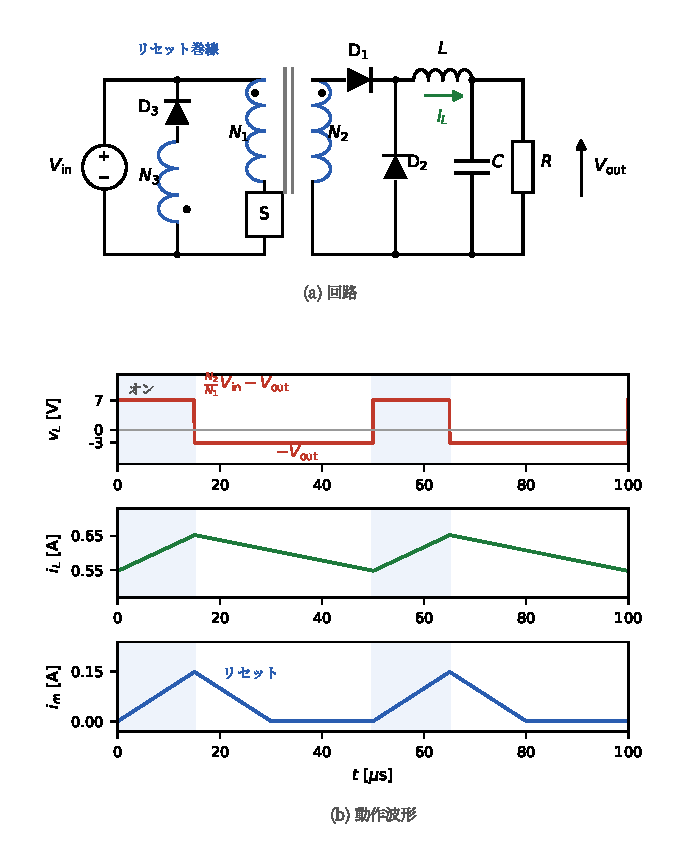
\includegraphics[clip]{figures/fig6.4.eps}
\end{center}
\caption{フォワードコンバータ。(a)回路。5章の降圧コンバータのスイッチの後ろに
変圧器を挟んだ形で，リセット巻線$N_3$が励磁エネルギーを電源へ返す。
(b)動作波形。$v_L$のボルト秒平衡は5章の降圧コンバータと同形で，
励磁電流$i_m$はオンで増えリセットでゼロに戻る}
\label{fig6.4}
\end{figure}

解析の仮定を明示する。
\textbf{スイッチとダイオードは理想}（電圧降下・切替え時間ゼロ），
\textbf{定常状態}（波形が周期$T$で繰り返す），
\textbf{リプルは小さい}（出力電圧はほぼ一定値$V_{\mathrm{out}}$），
インダクタ電流は連続（CCM），
そして\rev{\textbf{励磁電流は反射電流（1次側に映った負荷電流）に比べて小さく，電力の計算では無視する}}。

\subsection{オンとオフの2つの回路}

スイッチがオンの間（$0 \le t < DT$），1次巻線には$v_1 = V_{\mathrm{in}}$がかかり，
2次巻線には式\ref{eq6.3}より$v_2 = (N_2/N_1)V_{\mathrm{in}}$が現れる。
この電圧で$\mathrm{D_1}$が導通し，$\mathrm{D_2}$は逆バイアスされるから，
インダクタ$L$の左端は$(N_2/N_1)V_{\mathrm{in}}$，右端は$V_{\mathrm{out}}$である。
\begin{equation}
v_L = \frac{N_2}{N_1}V_{\mathrm{in}} - V_{\mathrm{out}} \qquad （オン期間）
\label{eq6.9}
\end{equation}

\rev{スイッチがオフの間（$DT \le t < T$），1次側の電流は断たれる。
後述のリセット期間には1次巻線に$-(N_1/N_3)V_{\mathrm{in}}$の負の電圧がかかるから，
2次巻線にも$-(N_2/N_3)V_{\mathrm{in}}$の負の電圧が現れ，$\mathrm{D_1}$は逆バイアスされて切れる。
リセットが済んで巻線電圧がゼロになった後も，$\mathrm{D_1}$を押し開ける電圧はない。
こうして$\mathrm{D_1}$が切れている間，
インダクタ電流は$\mathrm{D_2}$を通って還流する。5章の降圧コンバータと同じく}
\begin{equation}
v_L = -V_{\mathrm{out}} \qquad （オフ期間）
\label{eq6.10}
\end{equation}
である。

\subsection{ボルト秒平衡で出力電圧を求める}

定常状態では，インダクタ$L$の電圧の1周期平均はゼロである（5章）。
オン期間の電圧$\times$時間とオフ期間の電圧$\times$時間がつり合うから，
式\ref{eq6.9}，式\ref{eq6.10}より
\begin{equation}
\left(\frac{N_2}{N_1}V_{\mathrm{in}} - V_{\mathrm{out}}\right) DT = V_{\mathrm{out}}\,(1-D)\,T
\label{eq6.11}
\end{equation}
両辺を$T$で割って展開すると
\begin{eqnarray}
\frac{N_2}{N_1}V_{\mathrm{in}}D - V_{\mathrm{out}} D &=& V_{\mathrm{out}} - V_{\mathrm{out}} D \nonumber\\
\frac{N_2}{N_1}V_{\mathrm{in}}D &=& V_{\mathrm{out}} \nonumber
\end{eqnarray}
すなわち
\begin{equation}
V_{\mathrm{out}} = \frac{N_2}{N_1}\,D\,V_{\mathrm{in}}
\label{eq6.12}
\end{equation}
となる。非絶縁型の降圧コンバータの$V_{\mathrm{out}} = DV_{\mathrm{in}}$に巻数比$N_2/N_1$が掛かっただけである。
\textbf{大まかな電圧の変換は巻数比が，細かな調整はデューティ比が受け持つ}
という\ref{sec6.1}節の分担が，式の形にそのまま現れている。

\begin{例題}[フォワードコンバータの巻数比設計]
\label{rei6.2}
入力$V_{\mathrm{in}} = 100$\,Vから出力$V_{\mathrm{out}} = 5$\,Vを作るフォワードコンバータを設計する。
デューティ比を$D = 0.4$としたい。巻数比$N_1 : N_2$を求めよ。
\begin{解答}
式\ref{eq6.12}を巻数比について解くと
\begin{equation*}
\frac{N_2}{N_1} = \frac{V_{\mathrm{out}}}{D\,V_{\mathrm{in}}} = \frac{5}{0.4\times100} = \frac{1}{8}
\end{equation*}
よって$N_1 : N_2 = 8 : 1$である。
もし非絶縁型の降圧コンバータで作れば$D = 5/100 = 0.05$という極端な値になるが，
巻数比に$1/8$を受け持たせることで$D$は制御しやすい$0.4$に収まる。
\end{解答}
\end{例題}

\subsection{励磁電流のリセット ― 蓄えっぱなしは許されない}

ここまでの計算は理想変圧器（励磁電流ゼロ）で済んだ。
しかし実際には，オンのたびに励磁インダクタンス$L_m$へ$V_{\mathrm{in}}$がかかり，
励磁電流は式\ref{eq6.4}に従って$V_{\mathrm{in}}DT/L_m$ずつ増える。
オフの間にこの電流をゼロへ戻す道がなければ，
励磁電流は周期ごとに積み上がり，鉄心は数周期で磁気飽和してしまう。
$L_m$にもボルト秒平衡が必要なのに，
正の電圧しかかけていないからである。
フォワードコンバータのトランスは電力を素通しで渡すだけで，
励磁分のエネルギーを自分から吐き出すしくみを持たない。
そこで，励磁エネルギーの返却専用の経路を追加する。

\begin{定義}[リセット巻線]
\label{def6.3}
オフ期間に励磁電流を引き継ぎ，
励磁エネルギーを電源へ返すための第3の巻線（巻数$N_3$）を
\index{りせっとまきせん@リセット巻線}\textbf{リセット巻線}という。
直列のダイオード$\mathrm{D_3}$は，オン期間には逆バイアスで眠っていて，
オフ期間だけ導通する向きに入れる。
\end{定義}

オフ期間の動作を追う。スイッチが切れると，
励磁電流は行き場を求めて巻線電圧の向きを反転させ（4章のインダクタと同じ），
$\mathrm{D_3}$が導通する。するとリセット巻線は電源$V_{\mathrm{in}}$につながれ，
その電圧は$-V_{\mathrm{in}}$に固定される。1次側に換算すれば，$L_m$には
\begin{equation}
v_{Lm} = -\frac{N_1}{N_3}V_{\mathrm{in}} \qquad （リセット期間）
\label{eq6.13}
\end{equation}
がかかり，励磁電流は一定の傾きで減って，時間$t_r$後にゼロに達する。
$L_m$のボルト秒平衡から$t_r$が求められる。
\begin{equation}
V_{\mathrm{in}}\,DT = \frac{N_1}{N_3}V_{\mathrm{in}}\,t_r
\qquad\Rightarrow\qquad
t_r = \frac{N_3}{N_1}\,DT
\label{eq6.14}
\end{equation}
リセットはオフ期間内に完了しなければならない。
$t_r \le (1-D)T$に式\ref{eq6.14}を代入すると
\begin{equation}
\frac{N_3}{N_1}D \le 1-D
\qquad\Rightarrow\qquad
D \le \frac{1}{1 + N_3/N_1}
\label{eq6.15}
\end{equation}
という\textbf{デューティ比の上限}が現れる。
よく使われる$N_3 = N_1$では$D \le 0.5$である。
\ref{fig6.4}(b)の$i_m$の波形が，この「オンで蓄え，リセットで返す」
往復を示している。

\begin{注意}
リセット期間中，スイッチには$V_{\mathrm{in}}$より高い電圧がかかる（\rev{本節末の問}）。
また，どんな変圧器にも鉄心を通らずに漏れる磁束が少しあり，
\index{もれいんだくたんす@漏れインダクタンス}\textbf{漏れインダクタンス}として働く。
その蓄えたエネルギーはスイッチが切れた瞬間に行き場を失い，
サージ電圧を生む。実際の回路では，これを吸収する保護回路
（\index{すなばかいろ@スナバ回路}\textbf{スナバ回路}）を添えることが多い。
\end{注意}

\begin{問}
\item $N_3 = N_1$のフォワードコンバータで，リセット期間中に
スイッチの両端へかかる電圧が$2V_{\mathrm{in}}$になることを示せ。
（ヒント：スイッチの両端電圧は$V_{\mathrm{in}}$と1次巻線電圧の和である。）
\end{問}

\rev{以上がフォワードコンバータである。励磁エネルギーを邪魔者として電源へ返したこの回路に対し，次節はそれを主役に据える。}

%%======================================================================
\section{フライバックコンバータ ― トランスに溜めてから渡す}
\label{sec6.4}

\subsection{昇降圧コンバータのインダクタに巻線を足す}

フォワードでは励磁エネルギーは邪魔者で，返却専用の巻線まで用意した。
発想を逆転させて，\textbf{励磁インダクタンスへの蓄えをエネルギー伝達の主役}
にしたのが\index{ふらいばっくこんばーた@フライバックコンバータ}
\textbf{フライバックコンバータ}である（\FIGref{fig6.5}(a)）。
5章の昇降圧コンバータで「オンでインダクタに蓄え，オフで負荷へ放出」した，
あのインダクタに2次巻線を追加し，
蓄えるのは1次巻線から，取り出すのは2次巻線から，と分担させた回路である。
この使い方のトランスは，電力を素通しさせる変圧器というより
\textbf{2つの巻線を持つインダクタ（結合インダクタ）}と呼ぶ方が実態に近い。

\begin{figure}[ht]
\begin{center}
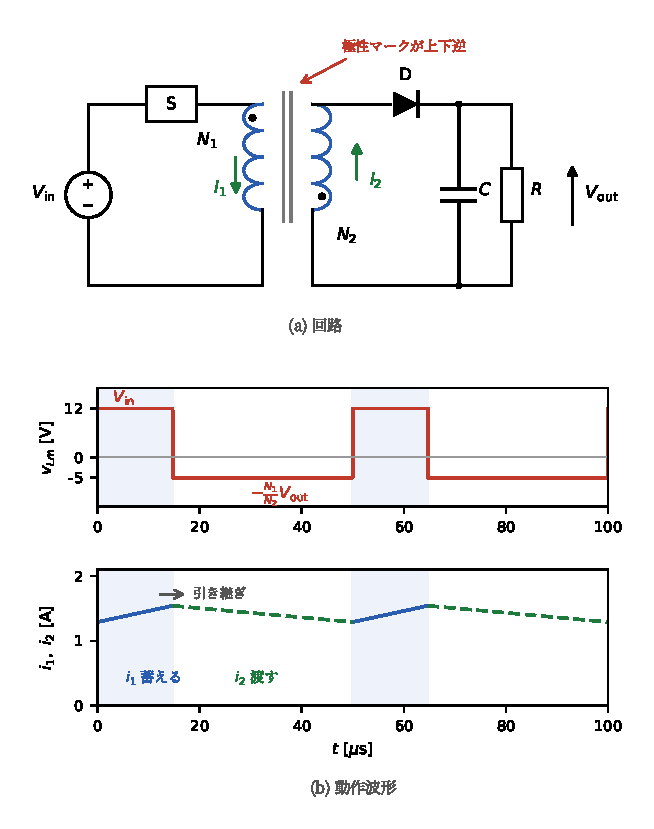
\includegraphics[clip]{figures/fig6.5.eps}
\end{center}
\caption{フライバックコンバータ。(a)回路。極性マークが上下逆であることに注意。
(b)動作波形。オン期間は1次電流$i_1$が励磁エネルギーを蓄え，
オフ期間は2次電流$i_2$がそれを負荷へ放出する。電流の受け渡しの瞬間，
巻数比に応じて値が飛ぶ}
\label{fig6.5}
\end{figure}

回路の要点は\textbf{極性マークの向き}である。
\ref{fig6.5}(a)では1次と2次のドットが互いに逆側に打たれ，
ダイオード$\mathrm{D}$は，オン期間に2次側へ電流が流れ出さない向きに入っている。
\rev{仮定は前節と同じく，理想素子・定常状態・小リプル（出力電圧はほぼ一定値$V_{\mathrm{out}}$），
そして\textbf{励磁電流は連続（CCM）}，すなわち$i_m$はオフ期間の終わりでもゼロに戻らないとする。
この最後の仮定が崩れる場合（DCM）については例題\ref{rei6.4}の後で触れる。}

\subsection{オンで蓄え，オフで渡す}

\textbf{オン期間}（$0 \le t < DT$）：
1次巻線すなわち励磁インダクタンス$L_m$に$V_{\mathrm{in}}$がかかり
\begin{equation}
v_{Lm} = V_{\mathrm{in}} \qquad （オン期間）
\label{eq6.16}
\end{equation}
励磁電流$i_m$（$=$1次電流$i_1$）は傾き$V_{\mathrm{in}}/L_m$で増える。
このとき2次巻線には，ドットの向きから$\mathrm{D}$を逆バイアスする電圧が現れるので，
2次電流は流れない。エネルギーは負荷へ渡らず，
すべて$\frac{1}{2}L_m i_m^2$として磁場に蓄えられる。
出力側では，キャパシタ$C$が蓄えた電荷で負荷電流を支えている。

\textbf{オフ期間}（$DT \le t < T$）：
スイッチが切れて1次電流の道が断たれると，
磁束を保とうとして巻線電圧が反転し（flyback＝跳ね返り），
今度は$\mathrm{D}$が導通して2次巻線から負荷へ電流が流れ出す。
切替えの瞬間，磁束（巻数$\times$電流）は連続だから，電流は
\begin{equation}
N_1 i_m = N_2 i_2
\qquad\Rightarrow\qquad
i_2 = \frac{N_1}{N_2}\,i_m
\label{eq6.17}
\end{equation}
と，1次から2次へ巻数比に応じて値を変えて引き継がれる（\ref{fig6.5}(b)）。
導通した$\mathrm{D}$を通じて2次巻線の電圧は出力電圧$V_{\mathrm{out}}$に固定されるから，
1次側に換算すると
\begin{equation}
v_{Lm} = -\frac{N_1}{N_2}V_{\mathrm{out}} \qquad （オフ期間）
\label{eq6.18}
\end{equation}
である。蓄えたエネルギーはこの間に負荷とキャパシタへ放出される。

\subsection{ボルト秒平衡で出力電圧を求める}

定常状態では$L_m$の電圧の1周期平均はゼロだから，
式\ref{eq6.16}，式\ref{eq6.18}より
\begin{equation}
V_{\mathrm{in}}\,DT = \frac{N_1}{N_2}V_{\mathrm{out}}\,(1-D)\,T
\label{eq6.19}
\end{equation}
両辺を$T$で割り，$V_{\mathrm{out}}$について解くと
\begin{eqnarray}
V_{\mathrm{in}}\,D &=& \frac{N_1}{N_2}V_{\mathrm{out}}\,(1-D) \nonumber\\
V_{\mathrm{out}} &=& \frac{N_2}{N_1}\cdot\frac{D}{1-D}\,V_{\mathrm{in}}
\label{eq6.20}
\end{eqnarray}
となる。\rev{非絶縁型の昇降圧コンバータの$|V_{\mathrm{out}}| = \frac{D}{1-D}V_{\mathrm{in}}$（式\ref{eq5.18}の大きさ）に}
巻数比が掛かった形で，$D < 0.5$で降圧，$D > 0.5$で昇圧になる。
しかも5章の昇降圧コンバータでは出力の極性が反転してしまったのに対し，
フライバックでは\textbf{巻線の向き（ドットの打ち方）で出力の極性を自由に選べる}。
極性の反転が絶縁で解消されるのである。

\rev{フォワードと違ってリセット巻線は要らない。
オン期間に蓄えた励磁エネルギーは，毎周期オフ期間に2次側へ放出されるからである
（CCMでは谷の分$\frac{1}{2}L_m I_{\min}^2$が残るが，これは周期ごとに積み上がるものではなく，定常的に持ち越される一定の蓄えである）。
「蓄えっぱなしにしない」というトランスの掟を，
フライバックはエネルギー伝達そのもので満たしている。}

\begin{例題}[フライバックコンバータの巻数比設計]
\label{rei6.3}
AC100\,Vを整流した$V_{\mathrm{in}} = 141$\,Vから$V_{\mathrm{out}} = 5$\,Vを作る
フライバックコンバータを，$D = 0.4$を中心に設計したい。
(a)巻数比$N_1/N_2$を求めよ。
(b)巻数比を整数比$19:1$に丸めたときの実際のデューティ比を求めよ。
\begin{解答}
(a) 式\ref{eq6.20}を巻数比について解くと
\begin{equation*}
\frac{N_1}{N_2} = \frac{D}{1-D}\cdot\frac{V_{\mathrm{in}}}{V_{\mathrm{out}}}
= \frac{0.4}{0.6}\times\frac{141}{5} \approx 18.8
\end{equation*}
(b) 巻数は整数だから$N_1 : N_2 = 19 : 1$に丸める。式\ref{eq6.20}より
\begin{equation*}
\frac{D}{1-D} = \frac{N_1}{N_2}\cdot\frac{V_{\mathrm{out}}}{V_{\mathrm{in}}}
= 19\times\frac{5}{141} \approx 0.674
\qquad\Rightarrow\qquad
D \approx 0.40
\end{equation*}
となり，ほぼ狙いどおりの$D$で動作できる。
$141$\,Vから$5$\,Vという28倍の変換でも，
巻数比が大部分を受け持つおかげで$D$は0.4に保てる。
ACアダプタや携帯機器の充電器で
フライバックが定番である理由がここにある。
\end{解答}
\end{例題}

\rev{巻数比が決まれば，次は5章と同じ手順で素子値を決める。
フライバックで決めるべきは，励磁インダクタンス$L_m$，そこから決まる電流の山$I_{\mathrm{pk}}$（スイッチとダイオードの定格），
そして出力キャパシタ$C$の3つである。}

\begin{例題}[フライバックコンバータの数値設計]
\label{rei6.4}
\rev{$V_{\mathrm{in}} = 12$\,Vから$V_{\mathrm{out}} = 5$\,V・$P_{\mathrm{out}} = 5$\,W（$I_{\mathrm{out}} = 1$\,A）を作るフライバックコンバータを，
巻数比$N_1 : N_2 = 1 : 1$，スイッチング周波数$f = 20$\,kHzで設計する。損失はないものとする。
(a)~デューティ比$D$と，オン期間中の励磁電流の平均値$I_m$を求めよ。
(b)~励磁電流のリプル（オン期間の増え幅）$\mathit{\Delta}I_m$を$I_m$の2割以下に抑える$L_m$を求めよ。
また標準値$L_m = 0.7$\,mHを選んだときの励磁電流の山$I_{\mathrm{pk}}$と谷$I_{\min}$を求め，CCMであることを確かめよ。
(c)~出力のリプル電圧を$\mathit{\Delta}V_{\mathrm{out}} = 50$\,mV（$V_{\mathrm{out}}$の1\,\%）以下にする$C$を求めよ。}
\begin{解答}
\rev{(a) 式\ref{eq6.20}に$N_2/N_1 = 1$を代入すると$D/(1-D) = 5/12$，よって$D = 5/17 \approx 0.294$である。
周期は$T = 1/f = 50\,\mathrm{\mu s}$，オン時間は$DT \approx 14.7\,\mathrm{\mu s}$になる。
損失がなければ入力電力は出力と同じ$5$\,Wだから，入力電流の平均は$I_{\mathrm{in}} = 5/12 \approx 0.417$\,Aである。
1次電流はオン期間にしか流れない（\ref{fig6.5}(b)）ので，オン期間中の励磁電流の平均$I_m$は}
\begin{equation*}
I_m = \frac{I_{\mathrm{in}}}{D} = \frac{0.417}{0.294} \approx 1.42\,\mathrm{A}
\end{equation*}
\rev{と，平均入力電流の$1/D$倍になる。}

\rev{(b) オン期間に$L_m$には$V_{\mathrm{in}}$がかかるから，式\ref{eq6.4}より
$\mathit{\Delta}I_m = V_{\mathrm{in}}\,DT/L_m$である。これを$0.2 I_m \approx 0.28$\,A以下にするには}
\begin{equation*}
L_m \ge \frac{V_{\mathrm{in}}\, DT}{\mathit{\Delta}I_m}
= \frac{12 \times 14.7\times10^{-6}}{0.28} \approx 0.63\,\mathrm{mH}
\end{equation*}
\rev{標準値$L_m = 0.7$\,mHを選ぶと
$\mathit{\Delta}I_m = 12\times14.7\times10^{-6}/(0.7\times10^{-3}) \approx 0.25$\,Aで，}
\begin{equation*}
I_{\mathrm{pk}} = I_m + \frac{\mathit{\Delta}I_m}{2} \approx 1.54\,\mathrm{A}，\qquad
I_{\min} = I_m - \frac{\mathit{\Delta}I_m}{2} \approx 1.29\,\mathrm{A}
\end{equation*}
\rev{となる。谷$I_{\min}$が正なので励磁電流はゼロに戻らず，CCMの仮定は満たされている。
\ref{fig6.5}(b)の波形は，まさにこの動作点を描いたものである。
2次電流の山は式\ref{eq6.17}より$(N_1/N_2)I_{\mathrm{pk}} \approx 1.54$\,Aで，スイッチもダイオード$\mathrm{D}$もこの値に余裕を見た電流定格で選ぶ。}

\rev{(c) オン期間は$\mathrm{D}$が切れて，負荷電流$I_{\mathrm{out}}$を$C$の放電だけが支える。
これは5章の昇圧・昇降圧コンバータと同じ状況だから，リプル電圧は式\ref{eq5.24b}で求まり，式\ref{eq5.25b}より}
\begin{equation*}
C \ge \frac{I_{\mathrm{out}}\, D}{f\, \mathit{\Delta}V_{\mathrm{out}}}
= \frac{1 \times 0.294}{20\times10^{3} \times 0.05} \approx 290\,\mathrm{\mu F}
\end{equation*}
\rev{標準値$C = 500\,\mathrm{\mu F}$を選べば$\mathit{\Delta}V_{\mathrm{out}} \approx 29$\,mVに収まる。
こうして決めた$L_m = 0.7$\,mH，$C = 500\,\mathrm{\mu F}$，$D = 0.294$は，章末問題\ref{ex6.5}のシミュレーションの定数そのものである。}
\end{解答}
\end{例題}

\rev{例題\ref{rei6.4}の動作点で，1周期に2次側へ渡るエネルギーを確かめておこう。
オン期間の終わりにトランスが蓄えているのは$\frac{1}{2}L_m I_{\mathrm{pk}}^2 \approx 0.83$\,mJだが，
CCMではオフ期間の終わりにも$\frac{1}{2}L_m I_{\min}^2 \approx 0.58$\,mJが残っている。
渡るのは差の$\frac{1}{2}L_m(I_{\mathrm{pk}}^2 - I_{\min}^2) \approx 0.25$\,mJで，
これに$f = 20$\,kHzを掛けると$5.0$\,W ― 出力電力と一致する。
CCMのフライバックが毎周期渡すのは「蓄えの全部」ではなく「蓄えの増減分」である。}

\rev{一方，負荷が軽くなるか$L_m$が小さいと，5章の降圧コンバータと同じく（\ref{sec5.7}節），
オフ期間の終わりに励磁電流がゼロに達して電流不連続モード（DCM）に入る。
実は，ACアダプタなどの小電力フライバックでは，あえてDCM，または谷がちょうどゼロに触れる境界で運転することが多い。
毎周期トランスが空になるので小さな$L_m$で済み（トランスが小型になる），
ダイオードは電流がゼロになってから切れるので逆回復（3章）の損失も出ないからである。
そのかわり，同じ電力を送るのに必要なピーク電流はCCMより大きく，
出力電圧も$D$だけでは決まらなくなる（\ref{sec5.7}節と同じ理屈）。
境界またはDCMで運転するときは蓄えの全部が毎周期渡るので，1周期に運ぶエネルギーは$W = \frac{1}{2}L_m I_{\mathrm{pk}}^2$，
送れる電力は$P = Wf$と簡単に書ける。次の問はこの場合の検算である。}

\begin{問}
\item \rev{励磁電流がオフ期間の終わりにちょうどゼロに戻る境界（またはDCM）で動作しているフライバックコンバータが，
オン期間の終わりに蓄えているエネルギーは
$W = \frac{1}{2}L_m I_{\mathrm{pk}}^2$であり，これを毎周期そっくり渡すときに送れる電力は
$P = W f$（$f = 1/T$はスイッチング周波数）である。
$W$と$P$の右辺の単位がそれぞれJとWになることを確かめよ。
インダクタンスの単位H $= \mathrm{V\cdot s/A}$を使ってよい。}
\end{問}

\subsection{通すか，溜めてから渡すか ― 2つの回路の対比}

\FIGref{fig6.6}に，本章の2つのコンバータのエネルギーの流れを対比して示す。
フォワードはオン期間に電源から負荷へエネルギーを\textbf{通す}回路で，
蓄積の主役は2次側のインダクタ$L$，トランスの蓄え（励磁）は
邪魔者としてリセット巻線で返却する。
フライバックはオン期間にトランスへ\textbf{溜め}，
オフ期間に\textbf{渡す}回路で，トランスの蓄えこそが主役である。
両者の特徴を\TABref{tab6.1}にまとめる。

\begin{figure}[ht]
\begin{center}
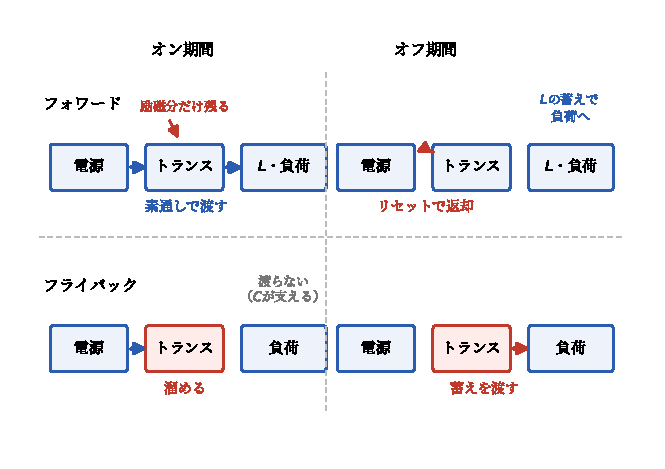
\includegraphics[clip]{figures/fig6.6.eps}
\end{center}
\caption{エネルギーの流れの対比。フォワードはオン期間にトランスを素通しで渡し
（励磁分だけはリセットで返却），フライバックはオン期間に溜めてオフ期間に渡す}
\label{fig6.6}
\end{figure}

\begin{table}[ht]
\begin{center}
\caption{フォワードコンバータとフライバックコンバータの対比}
\label{tab6.1}
\begin{tabular}{l|c|c}
\hline
 & フォワード & フライバック \\
\hline
エネルギーの渡し方 & オン期間に通す & オンで溜めオフで渡す \\
出力電圧 & $\dfrac{N_2}{N_1}DV_{\mathrm{in}}$（降圧） & $\dfrac{N_2}{N_1}\dfrac{D}{1-D}V_{\mathrm{in}}$（昇降圧） \\
トランスの蓄え & 小さく保つ（リセット） & 積極的に利用する \\
追加部品 & リセット巻線，$L$ & なし（出力は$C$のみ） \\
向く用途 & 中〜大電力 & 小電力（充電器など） \\
\hline
\end{tabular}
\end{center}
\end{table}

フライバックは部品が少なく小電力の絶縁電源で圧倒的に使われるが，
エネルギーを一度全部トランスに積むため，
電力が大きくなるとトランスとリプルが急速に大きくなる。
大電力ではオン期間中も電力が流れ続けるフォワード（とその発展形）が有利になる。
どちらを選ぶかは「どこにエネルギーを蓄え，いつ放出するか」の選択そのものである。

次章では，スイッチングをやめて損失で電圧を落とす対極の方式 ―
リニアレギュレータ ― を扱い，スイッチング方式の意味をあらためて見つめ直す。

%%======================================================================
\begin{章末問題}
\item \label{ex6.1}
入力$48$\,V，巻数比$N_1:N_2 = 6:1$，デューティ比$D = 0.375$，
スイッチング周波数$f = 100$\,kHzのフォワードコンバータ
（$N_3 = N_1$）がある。
\begin{enumerate}
\item[(a)] 出力電圧$V_{\mathrm{out}}$を求めよ。
\item[(b)] オフ期間のインダクタ電圧が$-V_{\mathrm{out}}$であることを使い，
インダクタ電流のリプル（増減幅）を$\mathit{\Delta}I_L = 0.2$\,A以下に
抑えるためのインダクタンス$L$の条件を求めよ。
\end{enumerate}

\item \label{ex6.2}
リセット巻線を$N_3 = N_1/2$としたフォワードコンバータについて答えよ。
\begin{enumerate}
\item[(a)] デューティ比の上限を式\ref{eq6.15}から求めよ。
\item[(b)] リセット期間中にスイッチへかかる電圧を$V_{\mathrm{in}}$で表せ。
\item[(c)] $N_3$を小さくすることの利点と代償を1行ずつ述べよ。
\end{enumerate}

\item \label{ex6.3}
$V_{\mathrm{in}} = 12$\,Vのバッテリーから絶縁した出力を作る
フライバックコンバータについて答えよ。
\begin{enumerate}
\item[(a)] $N_1:N_2 = 1:1$で$V_{\mathrm{out}} = 12$\,Vを得るためのデューティ比$D$を求めよ。
\item[(b)] $N_1:N_2 = 1:2$で$V_{\mathrm{out}} = 48$\,Vを得るためのデューティ比$D$を求めよ。
\end{enumerate}

\item \label{ex6.4}
$V_{\mathrm{in}} = 100$\,V，$L_m = 10$\,mH，$D = 0.3$，$f = 20$\,kHz，
$N_3 = N_1$のフォワードコンバータについて答えよ。
\begin{enumerate}
\item[(a)] オン期間の終わりの励磁電流のピーク値を求めよ。
\item[(b)] そのときトランスに蓄えられているエネルギーを求めよ。
\item[(c)] リセットに要する時間を求め，オフ期間内に完了することを確かめよ。
\item[(d)] もしリセット巻線のダイオードが断線したら，励磁電流は
周期ごとにどれだけ増え続けるか。何が起こるかを述べよ。
\end{enumerate}

\item \label{ex6.5}
\rev{（LTspiceで確かめよ）結合インダクタ（\texttt{K1 L1 L2 1}）を使って
フライバックコンバータ（$V_{\mathrm{in}} = 12$\,V，$L_1 = L_2 = 0.7$\,mH，
$C = 500$\,$\mu$F，$R = 5$\,$\Omega$，$f = 20$\,kHz，$D = 0.2941$。
例題\ref{rei6.4}の設計値であり，配布モデル\texttt{chapter06/flyback\_converter.asc}と同一）を組み，
シミュレーションで確かめよ。}
\begin{enumerate}
\item[(a)] 出力電圧の平均値を式\ref{eq6.20}の理論値と比較せよ。
\item[(b)] 入力電圧も同時に変えて，次の3ケースで降圧・等倍・昇圧の3つの動作を確認せよ：
$D = 0.2941$・$V_{\mathrm{in}} = 12$\,V（降圧，$V_{\mathrm{out}} \approx 5$\,V），
$D = 0.5$・$V_{\mathrm{in}} = 12$\,V（等倍，$V_{\mathrm{out}} \approx 12$\,V），
$D = 0.7059$・$V_{\mathrm{in}} = 5$\,V・$R = 28.8$\,$\Omega$（昇圧，$V_{\mathrm{out}} \approx 12$\,V）。
\item[(c)] 1次電流と2次電流の波形を重ねて表示し，
スイッチが切れる瞬間に電流が1次から2次へ引き継がれること
（式\ref{eq6.17}）を確かめよ。
\end{enumerate}
\end{章末問題}
